% Please make sure you insert your
% data according to the instructions in PoSauthmanual.pdf
\documentclass[a4paper,11pt]{article}
\usepackage{pos}
\usepackage{wrapfig}
\usepackage{svg}
\usepackage{lineno}

\linenumbers

\title{MLMC: Machine Learning Monte Carlo for Lattice Gauge Theory}
%% \ShortTitle{Short Title for header}

\author*[a]{Sam Foreman}
\author[a,b]{Xiao-Yong Jin}
\author[a,b]{James C. Osborn}

\affiliation[a]{Leadership Computing Facility, Argonne National Laboratory,\\
  9700 S. Cass Ave, Lemont IL, USA}

\affiliation[b]{Computational Science Division, Argonne National Laboratory,\\
9700 S. Cass Ave, Lemont IL, USA}

\emailAdd{foremans@anl.gov}
\emailAdd{xjin@anl.gov}
\emailAdd{osborn@alcf.anl.gov}

\abstract{%
  We present a trainable framework for efficiently generating gauge
configurations, and discss ongoing work in this direction. In particular, we
consider the problem of sampling configurations from a 4D $SU(3)$ lattice gauge
theory, and consider a generalized leapfrog integrator in the molecular
dynamics update that can be trained to improve sampling efficiency.%
}

\FullConference{The 40th International Symposium on Lattice Field Theory (Lattice 2023)\\
July 31st - August 4th, 2023\\
Fermi National Accelerator Laboratory\\}

%% \tableofcontents

\begin{document}
\maketitle


\section{\label{sec:intro}Introduction}

\section{\label{sec:background}Background}

We would like to calculate observables $\mathcal{O}$:
%
\begin{equation}
\left\langle \mathcal{O}\right\rangle \propto \int \left[\mathcal{D} x\right]\, \mathcal{O}(x)\, p(x)
\end{equation}
%
If these were independent, we could approximate the integral as $\left\langle\mathcal{O}\right\rangle \simeq \frac{1}{N}\sum_{n=1}^{N} \mathcal{O}(x_{n})$ with variance
%
\begin{equation}
\sigma_{\mathcal{O}}^{2} = \frac{1}{N}\,\mathrm{Var}\left[\mathcal{O}(x)\right] \Longrightarrow \sigma_{\mathcal{O}} \propto \frac{1}{\sqrt{N}}.
\end{equation}
%
Instead, nearby configurations are correlated, causing us to incur a factor of $\tau_{\mathrm{int}}^{\mathcal{O}}$ in the variance expression
%
\begin{equation}
\sigma_{\mathcal{O}}^{2} = \frac{\tau_{\mathrm{int}}^{\mathcal{O}}}{N} \mathrm{Var}\left[\mathcal{O}(x)\right]
\end{equation}


\subsection{\label{subsec:hmc}Hamiltonian Monte Carlo (HMC)}
%
We can use the Hamiltonian Monte Carlo (HMC) algorithm to help reduce these auto-correlations.
%
Specifically, we want to (sequentially) construct a chain of states:
%
\begin{equation}
x_{0} \rightarrow x_{1} \rightarrow x_{i} \rightarrow \cdots \rightarrow x_{N}
\end{equation}
%
such that, as $N \rightarrow \infty$:
%
\begin{equation}
\left\{x_{i}, x_{i+1}, x_{i+2}, \ldots, x_{N}\right\} \xrightarrow[]{N\rightarrow\infty} p(x)
\end{equation}
%
To do this, we begin by introducing a fictitious momentum\footnote{Here $\sim$ means \textit{is distributed according to}.} $v \sim \mathcal{N}(0, 1)$ normally distributed, independent of $x$.
%
We can write the joint distribution $p(x, v)$ as
%
\begin{align}
p(x, v) &= p(x) p(v) \propto e^{-S(x)} e^{-\frac{1}{2} v^{T}v} \\
&= e^{-\left[S(x) + \frac{1}{2} v^{T} v \right]} \\
&= e^{-H(x, v)}
\end{align}
%
We can evolve the Hamiltonian dynamics of the $(\dot{x}, \dot{v}) = (\partial_{v} H, -\partial_{x} H)$ system using operators $\Gamma: v \rightarrow v'$ and $\Lambda: x \rightarrow x'$.
%
Explicitly, for a single update step of the leapfrog integrator:
%
\begin{align}
\tilde{v} &\coloneqq \Gamma(x, v) = v - \frac{\varepsilon}{2} F(x) \\
x' &\coloneqq \Lambda(x, \tilde{v}) = x + \varepsilon \tilde{v} \\
v' &\coloneqq \Lambda(x', \tilde{v}) = \tilde{v} - \frac{\varepsilon}{2} F(x'),
\end{align}
%
where we've written the force term as $F(x) = \partial_{x}S(x)$.
%
Typically, we build a trajectory of $N_{\mathrm{LF}}$ leapfrog steps
%
\begin{equation}
(x_{0}, v_{0}) \rightarrow (x_{1}, v_{1}) \rightarrow \cdots \rightarrow (x', v'),
\end{equation}
%
and propose $x'$ as the next state in our chain.
%
This proposal state is accepted according to the Metropolis-Hastings criteria~\cite{mh}.
%
\begin{equation}
A(x'|x) = \mathrm{min}\left\{{1, \frac{p(x')}{p(x)} \left| \frac{\partial x'}{\partial x} \right|}\right\}.
\end{equation}
%
\section{\label{sec:method}Method}
%
\begin{wrapfigure}[22]{r}{0.5\textwidth}
  \begin{center}
  %\vspace{-25pt}
    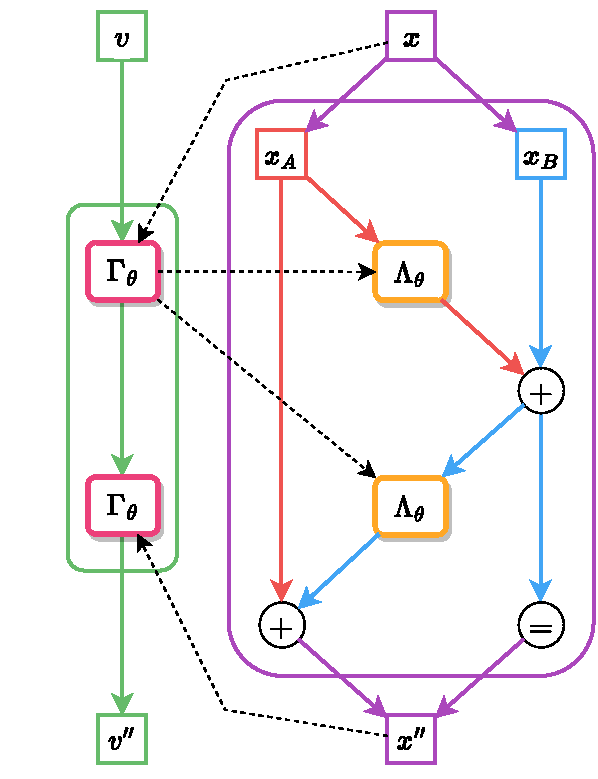
\includegraphics[width=\linewidth]{assets/leapfrog-layer-alt-2}
  \end{center}
  \caption{\label{fig:lf-layer}Illustration of the generalized MD update $\texttt{leapfrog layer}: (x, v) \rightarrow (x'', v'')$.}
\end{wrapfigure}
%
Unfortunately, HMC is known to suffer from long auto-correlations and often struggles with multi-modal target densities.
%
Instead, we propose building on the approach from~\cite{L2HMC,FTHMC,etc}. We introduce two (invertible) neural networks (\texttt{xNet}, \texttt{vNet}):
%
\begin{align}
\texttt{vNet}&: (x, F) \rightarrow (s_{v}, t_{v}, q_{v}) \\
\texttt{xNet}&: (x, v) \rightarrow (s_{x}, t_{x}, q_{x})
\end{align}
%
where $s, t, q$ are all of the same dimensionality as $x$ and $v$, and are parameterized by a set of weights $\theta$.
%
These network outputs $(s, t, q)$ are then used in a generalized MD update (as shown in Fig~\ref{fig:lf-layer}) via:
%
\begin{align}
\Gamma^{\pm}_{\theta}&: (x, v) \rightarrow (x, v') \\
\Lambda^{\pm}_{\theta}&: (x, v) \rightarrow (x', v).
\end{align}
%
where the superscript $\pm$ on $\Gamma^{\pm}_{\theta}, \Lambda^{\pm}_{\theta}$ correspond to the direction $d \sim \mathcal{U}(-1, +1)$ of the update\footnote{This can be \textit{absorbed} by constructing trajectories of $n$ forward $(+)$ steps followed by $n$ backward $(-)$ steps. See Appendix XXX for details.}.
%

To ensure that our proposed update remains reversible, we split the $x$ update into two sub-updates on complementary subsets ($x = x_{A} \cup x_{B}$):
%
\begin{align}
v' &= \Gamma_{\theta}(x, v) \\
x' &= x_{B} + \Lambda_{\theta}(x_{A}, v') \\
x'' &= x'_{A} + \Lambda_{\theta}(x'_{B}, v') \\
v'' &= \Gamma_{\theta}(x'', v')
\end{align}
%
%where $v_{0} \sim \mathcal{N}(0, 1)$ is re-sampled at the beginning of each trajectory and projected away at the end to obtain the proposal state $x'$.
%
\subsection{\label{subsec:algorithm}Algorithm}
\begin{enumerate}
    \item \texttt{input:} $x$
    \begin{itemize}
        \item Re-sample $v \sim \mathcal{N}(0, 1)$
        \item Construct initial state $\xi \coloneqq (x, v)$
    \end{itemize}
    \item \texttt{forward:} Generate proposal $\xi'$ by passing initial $\xi$ through $N_{\mathrm{LF}}$ leapfrog layers:
    \begin{equation}
        \xi \xrightarrow[]{\mathrm{LF\,\,\, Layer}} \xi_{1} \rightarrow \cdots \rightarrow \xi_{N_{\mathrm{LF}}} = \xi' \coloneqq (x'', v'')
    \end{equation}
    \begin{itemize}
        \item Metropolis-Hastings accept / reject:
        \begin{equation}
            A(\xi'|\xi) = \mathrm{min}\left\{1, \frac{\pi(\xi')}{\pi(\xi)} \left|\mathcal{J}\left(\xi', \xi\right)\right|\right\},
            \label{eq:MH}
        \end{equation}
        where $\left|\mathcal{J}(\xi',\xi)\right|$ is the determinant of the Jacobian.
    \end{itemize}
    \item \texttt{backward:} (if training)
    \begin{itemize}
        \item Evaluate the loss function $\mathcal{L}(\xi', \xi)$ and back propagate
    \end{itemize}
    \item \texttt{return:} $x_{i+1}$
    \begin{itemize}
        \item Evaluate MH criteria (Eq. ~\ref{eq:MH}) and return accepted config:
        \begin{equation}
            x_{i+1} \gets \begin{cases}
                x'' \quad \text{w/ prob.}\quad A(\xi'|\xi)  \\
                x \,\,\,\quad \text{w/ prob.} \quad 1 - A(\xi'|\xi)
            \end{cases}
        \end{equation}
    \end{itemize}
\end{enumerate}
%
\subsection{\label{subsec:4dSU3}4D \texorpdfstring{$SU(3)$}{SU(3)} Model}
%
\begin{wrapfigure}[23]{R}{0.4\textwidth}
  \begin{center}
    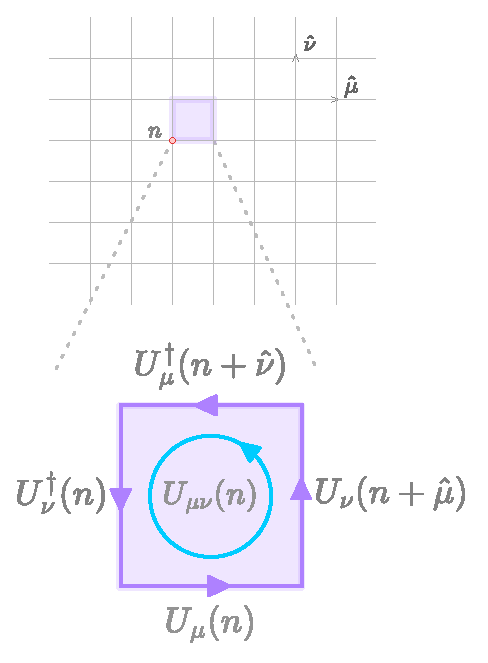
\includegraphics[width=0.4\textwidth]{assets/lattice}
  \end{center}
  \caption{Illustration of the lattice}
  \label{fig:lattice}
\end{wrapfigure}
%
Write link variables $U_{\mu}(x) \in SU(3)$:
%
\begin{align}
U_{\mu}(x) &= \exp\left[i \omega_{\mu}^{k}(x) \lambda^{k} \right] \\
&= e^{iQ}, \quad Q \in \mathfrak{su}(3)
\end{align}
%
where $\omega_{\mu}^{k}(x) \in \mathbb{R}$ and $\lambda^{k}$ are the generators of $SU(3)$.
%
We consider the standard Wilson gauge action
%
\begin{equation}
S_{G} = -\frac{\beta}{6}\sum \mathrm{Tr}\left[U_{\mu\nu}(x) + U^{\dagger}_{\mu\nu}(x) \right]
\end{equation}
%
where $U_{\mu\nu}(x) = U_{\mu}(x) U_{\nu}(x + \hat{\mu}) U_{\mu}^{\dagger}(x + \hat{\nu}) U^{\dagger}_{\nu}(x)$.
%

As before, we introduce momenta $P_{\mu}(x) = P^{k}_{\mu}(x) \lambda^{k}$ conjugate to the real fields $\omega_{\mu}^{k}(x)$.
%
We can write the Hamiltonian as
%
\begin{equation}
    H[P, U] = \frac{1}{2} P^{2} + S_{G}[U]
\end{equation}
%
by Hamilton's equations
%
\begin{equation}
\frac{d\omega^{k}}{dt} = \frac{\partial H}{\partial P^{k}},
\quad \frac{dP^{k}}{dt} = - \frac{\partial H}{\partial \omega^{k}}.
\end{equation}
%
To update the gauge field $U$,
%
\begin{equation}
    \frac{d\omega^{k}}{dt}\lambda^{k} = P^{k} \lambda^{k} \Rightarrow \frac{dQ}{dt} = P
\end{equation}
%
Discretizing with step size $\varepsilon$,
%
\begin{align}
    Q(\varepsilon) &= Q(0) + \varepsilon P(0) \Rightarrow \\
    -i \log U(\varepsilon) &= - i \log U(0) + \varepsilon P(0) \\
    U(\varepsilon) &= e^{i \varepsilon P(0)} U(0) \Longrightarrow \\
    \Lambda: U \rightarrow U' &\coloneqq e^{i\varepsilon P'} U.
\end{align}
%
and similarly for the momentum update,
%
\begin{align}
    \frac{dP^{k}}{dt} = - \frac{\partial H}{\partial \omega^{k}} &= - \frac{\partial H}{\partial Q} = - \frac{dS}{dQ} \Rightarrow \\
    P(\varepsilon) &= P(0) - \varepsilon \left.\frac{dS}{dQ}\right|_{t=0} \\
    &= P(0) - \varepsilon F[U] \\
    \Gamma: P \rightarrow P' &\coloneqq P - \frac{\varepsilon}{2} F[U],
\end{align}
%
where $F[U]$ is the force term.
%
In this case, our $\texttt{vNet}: (U, F) = (e^{iQ}, F) \rightarrow (s_{P}, t_{P}, q_{P})$.
%
We can use this in the momentum update $\Gamma^{\pm}_{\theta}$ via
\begin{enumerate}
    \item \texttt{forward}, $(+)$:
    \begin{equation}
        \Gamma^{+}(U, F) = P \cdot e^{\frac{\varepsilon}{2} s_{P}} - \frac{\varepsilon}{2}\left[ F \cdot e^{\varepsilon q_{P}} + t_{P} \right]
    \end{equation}
    \item \texttt{backward}, $(-)$:
    \begin{equation}
        \Gamma^{-}(U, F) = e^{-\frac{\varepsilon}{2} s_{P}} \left\{P + \frac{\varepsilon}{2} \left[ F \cdot e^{\varepsilon q_{P}} + t_{P} \right] \right\}
    \end{equation}
\end{enumerate}
%

\begin{thebibliography}{99}
\bibitem{...}
....

\end{thebibliography}

\end{document}
